\chapter{The D-Wave Quantum Computer}


TODO: intro del capítulo


\section{Quantum Annealing}


Simulated annealing (SA) is an general optimization technique that was first introduced in 1983 by Kirkpatrick \emph{et al.} \cite{Kirkpatrick1983}. The main idea is to mimic how thermal fluctuations work to let the system escape from local minimums in the cost function. The \emph{temperature} of the system dictates the probability with which the is allowed to jump to worse solutions (higher values of the cost function). The \emph{annealing schedule} is the decrease rate of the temperature, controlled by the programmer. Under the appropiate one, the system would be able to scape from local minimums to reach the global one. If the temperature decreases too quickly, the system converges prematurely to a local minimum. If it decreases too slowly, the technique transforms into a random walker, reaching the global minimum at some point but being worthless time-wise.

Inspiration in thermal fluctuations are used in SA so the system may escape from local minima. Similarly, \emph{quantum tunneling} is used in Quantum Annealing (QA) in order to escape from local minimums. This new technique was introduced in its present form by two similar proposals \cite{Finnila1994} \cite{Kadowaki1998}.

Quantum tunneling is a quantum mechanical phenomenon where a wavefunction (i.e. a quantum state) may propagate through a potetial barrier \cite{Nimtz2008}. The probability of this event occuring depends on the height and width of the barrier (see figure \ref{fig 2.1})

\begin{figure}[h]
	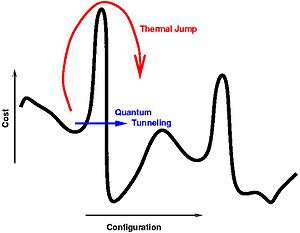
\includegraphics[scale=.8]{QuantumTunneling.jpg}
	\centering
	\caption{Thermal jumps vs quantum tunneling.}
	\label{fig 2.1}
\end{figure}

The main advantage of quantum tunneling compared to classical thermal fluctuations is that the probability of the system shifting depends to only on the height of the potential barrier but also on its width. Thus, application of QA may pottentially outperform SA in problems where the energy (cost) landscape consists on very high and thin barries surronding local minimums. 

Particularly, as studied in \cite{Ray1989}, let $\Delta$ be the height of a barrier and $\omega$ its width. The probability of a thermal transition ocurring is dictated by $exp\{-\frac{\Delta}{k_B T}\}$ where $T$ y the temperatue of the system and $k_B$ is the Boltzmann constant. On the other hand, the probability of a quantum tunneling transition ocurring through the same barrier (asumming isolation) is $exp\{-\frac{\sqrt \Delta \omega}{\Gamma}\}$, where $\Gamma$ is the tunneling field. Thus, the probability is much higher for the quantum tunneling effect on a high and thin barriers.

We may also observe looking at the previous expressions how the tunneling field and the temperature play a similar roles in the different methods. Thus, the annealing schedule of the QA system is controlled using the tunneling field just like the temperature is used in SA.

There are many examples in the literature of QA simulations using classical computers, both theoretical \cite{Morita2008} and numerical -most of them using Quantum Monte Carlo (QMC) methods \cite{Isakov2016} \cite{Farhi2000}-. This evidence suggests outperformance of SA by simulated QA under certain conditions. It is resonable to wonder what happens if instead of simulating QA we could somehow encode our problems in a real physical system that tends to its lower energy state (ground state), thus using quantum tunneling naturally. This is precisely what the D-Wave system does.

Let us farther deepen into the technicalities of quantum annealing in order to understand how it is implemented in the D-Wave system.


\section{Adiabatic Evolution}


The alternative form of the third postulate of quantum mechanics (section \ref{postulate-3'}) stated that the evolution of a quantum system is described by the Schrodinger equation:

$$ i \hbar \frac{d|\varphi\ra}{dt} = H|\varphi\ra $$

By better understanding the Hamiltonian $H$ we may controll this evolution. Suppose that at the evolution of a given quantum system is described by a Hamiltonian $\hat H(t)$. Suppose that at some initial time $t_0$ our quantum system is in an eigenstate $|\varphi(t_0)\ra$ of $\hat H(t_0)$. Since the evolution is continuous, at some other time $t_1 > t_0$ we could expect our system to be in the corresponding eigenstate $|\varphi(t_1)\ra$ of $\hat H(t_1)$. This fact critically depends on the time $\tau = t_1 - t_0$ during which the modification takes places, as stated by the adiabatic theorem, first proposed by Max Born and Vladimir Fock (1928) \cite{Born1928}.

\begin{theorem}[Adiabatic Theorem]
\label{adiabatic-theorem}
	A physical system remains in its instantaneous eigenstate if a given perturbation is acting on it slowly enough and if there is a gap between the eigenvalue and the rest of the Hamiltonian's spectrum.
\end{theorem}

Thus, we may define diabatic and adiabatic processes depending on how they adapt to the system changes \cite{Kato1950}.

\begin{definition}
	A \emph{diabatic process} is a process where rapidly changing conditions prevent the system from adapting its configuration during the process. Typically there is no eigenstate of the final Hamiltonian with the same functional form as the initial state. The system ends in a linear combination of the states.
\end{definition}

\begin{definition}
	An \emph{adiabatic process} is a process where gradually changing conditions allow the system to adapt its configuration. If the system starts in an eigenstate of the initial Hamiltonian, it will end in the corresponding eigenstate of the final Hamiltonian.
\end{definition}

The 'gap condition' that appears in theorem \ref{adiabatic-theorem} refers to an additional requiremente: the spectrum of $\hat H(t)$ is \emph{nondegenerate}, meaning there are no two equal eigenvalues at fixed time $t$. This condition is also called the \emph{no-crossing} condition, and allow us to sort the eigenstates using the eigenvalues without any ambiguity.

As a classical annalogy, consider a simple pendulum. If the pendulum's support point is moved, the oscillation of the pendulum may change. In fact, violent changes on the support point will dramatically affect the pendulum's movement, changing it completely. However, if the support point is moved slowly enough, the pendulum will remain unchange. These are examples of diabatic and adiabatic processes respectively.


\subsection{Avoided crossing}


Let us consider a important physical example known as the \emph{avoided crossing}. Consider a two-state quantum system, i.e. a qubit. Suppose its Hamiltonian to be:

$$
	H = 
	\begin{pmatrix}
		E_1 & 0 \\
		0 & E_2 
	\end{pmatrix}
$$

Whose eigenvalues are $E_1$ and $E_2$, and eigenvectors,

$$
	|0\ra = 
	\begin{pmatrix}
	1 \\
	0 
	\end{pmatrix}, \quad
	|1\ra = 
	\begin{pmatrix}
	0 \\
	1 
	\end{pmatrix}
$$

which will be used as our base. Thus, a state vector describing the system may be written as a superposition of both states:

$$ |\varphi\ra = \alpha(t)|0\ra + \beta(t)|1\ra $$

Supposing adiabatic evolution, if the system is prepared in either one of the eigenstates it will remain as such as long as the gap condition is suffied: $E_1 \neq E_2$. However, if $E_1 = E_2$, any superposition of states will be an eigenstate, thus remaining unchanged. Hence, independently of $E_1$ and $E_2$, any system prepared in an eigenstate will remain as such, supposed adiabatic evolution.

Let us consider a $P$ perturbation into our original system. For simplicity we only consider perturbations with degenerated diagonal. Our new Hamiltonian will be the following:

$$
	H' = H + P =
	\begin{pmatrix}
	E_1 & 0 \\
	0 & E_2 
	\end{pmatrix} +
	\begin{pmatrix}
	0 & \omega \\
	\overline \omega & 0 
	\end{pmatrix} = 
	\begin{pmatrix}
	E_1 & \omega \\
	\overline \omega & E_2 
	\end{pmatrix}
$$

where $\omega \in \C$. Note that by setting $\omega$, the other value in the antidiagonal is fixed since $H'$ must be Hermitian. By using the characteristic equation we may compute $H'$ eigenvectors:

$$ E_+ = \frac{1}{2}(E_1 + E_2) + \frac{1}{2}\sqrt{(E_1 - E_2)^2 + 4|\omega|^2} $$
$$ E_- = \frac{1}{2}(E_1 + E_2) - \frac{1}{2}\sqrt{(E_1 - E_2)^2 + 4|\omega|^2} $$

TODO1: Calcular a mano los eigenvalues y vectors a mano,
TODO2: Explicar que pasa cuando variamos ($E_1 - E_2$) y pintarlo en geogebra bonito
TODO3: Conclusion: en un qubit siempre se da el gap.
TODO4: Explicar que pasa en evolucion no adiabatica.

TODO: añadir autoria a las imagenes


\section{QUBO and Ising problems}

\subsection{example 1}
\subsection{example 2}
\subsection{example 3}

TODO: completar sección





\section{D-Wave Systems}


\textbf{D-Wave Systems Inc.} is a Canadian company dedicated to quantum computing. In 2011, they announced the first commercial quantum computer system, D-Wave One. During the following two decades, the D-Wave team have developed a series of computing computers dedicated to quantum annealing. The last one being the Advantage System (figure \ref{fig 2.2}).

\begin{figure}[h]
	\includegraphics[scale=.1]{advantage_system.png}
	\centering
	\caption{Advantage$^{TM}$ system}.
	\label{fig 2.2}
\end{figure}

The quantum processing unit (QPU) of this system consist of $5640$ qubits and $40,484$ \emph{couplers} (links between qubits that allow entanglement between a pair of qubits). The number of couplers is especially relevant. It tells us that not every qubit can be entangled with every other qubit. We will come back to this in section [TODOref]. Since the QPU must be isolated to operate, it is encapsulated in a system at temperatures below 15 mK. In addition, radio frequency (RF)-shielded enclousre and magnetic shieldings are used to protect it from electromagnetic interferience \cite{DWaveDoc}.

\begin{figure}[h]
	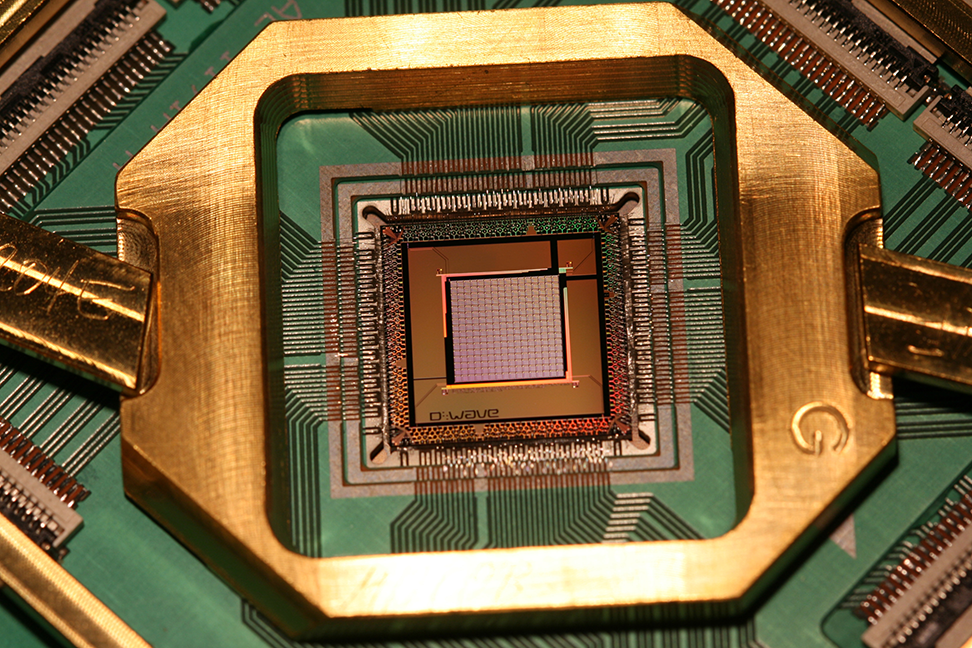
\includegraphics[scale=.2]{qpu.png}
	\centering
	\caption{D-Wave QPU}.
	\label{fig 2.3}
\end{figure}

D-Wave provides an easy-to-use software enviroment to solve problems using quantum annealing. We will explain in depth in section [TODOref].


\subsection{Quantum Annealing in D-Wave}
\label{quantum-annealing-dwave}


For this section we refer to the D-Wave documentation, which explains how quantum annealing is implemented and may be exploited in the D-Wave systems \cite{DWaveDoc-QuantumAnnealing}.




TODO: rephrasear la cita en el contexto anterior











https://journals.aps.org/prl/pdf/10.1103/PhysRevLett.117.180402




